در این مسائل هر state از خود مسئله یک جواب کامل است و اطلاعات لازم برای کل راه حل را دارا است.
نمونه‌هایی از این مسائل N-queen و TSP می‌باشد. (البته مسئله TCP را می‌توان به هر دو صورت بررسی نمود)

در این شکل از مسائل نیاز نیست تا زنجیره‌ای از state ها در حافظه قرار داشته باشند و می‌توان با داشتن یک state از مسئله و با کمک الگوریتم‌های local search به state بهتری دست پیدا کرد.
\begin{figure}[H]
    \minipage{0.4\textwidth}
    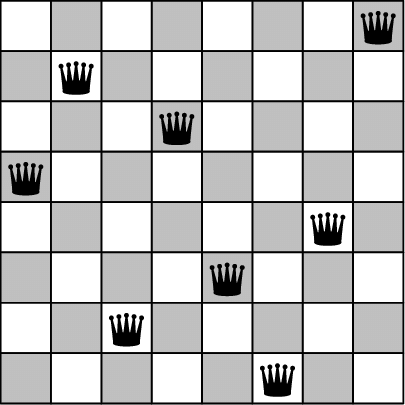
\includegraphics[width=\linewidth]{source/N-queen.png}
    \label{fig:HDD-to-Drive}
    \endminipage\hfill
    \minipage{0.4\textwidth}
    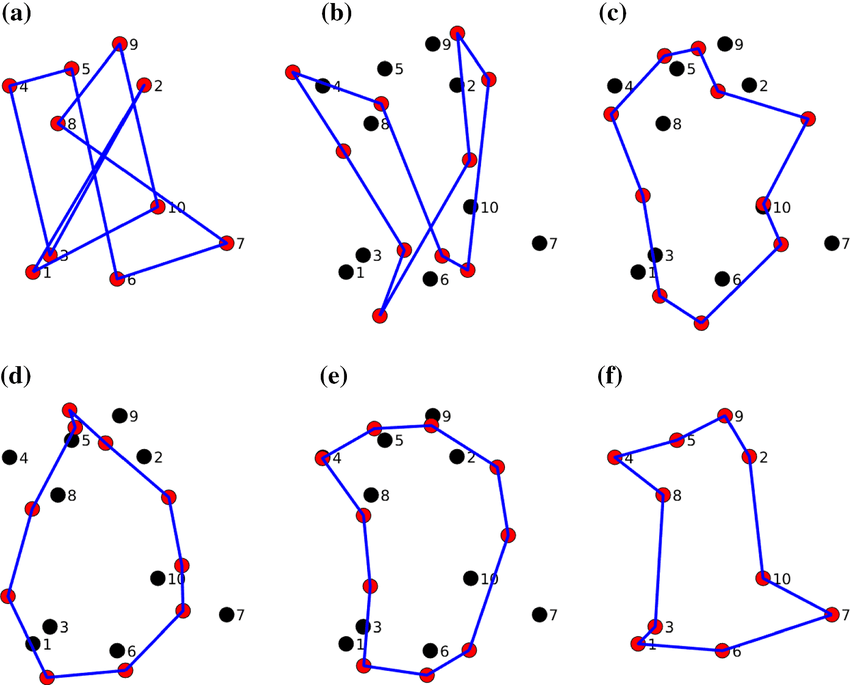
\includegraphics[width=\linewidth]{source/TSP.png}
    \label{fig:SSD-to-Drive}
    \endminipage\hfill
\end{figure}

البته باید اشاره کرد که با توجه به NP بودن مسئله TSP، هدف از الگوریتم بهینه‌سازی است در صورتی که در مسئله 8 وزیر، به دنبال یک هدف مشخص هستیم(هیچ یک از وزرا دیگری را تهدید نکند).
مسائلی مانند 8 وزیر را ‌توانیم با تعریف یک تابع heuristic به مسائلی مشابه با بهینه‌سازی تبدیل کنیم.
به طور مثال می‌توانیم تابع h را اینگونه تعریف کینم: تعداد وزرایی که یکدیگر را تهدید می‌کنند و سپس سعی کنیم تا این تابع را به کمینه مقدار خود که در مسئله 0 است، برسانیم.






